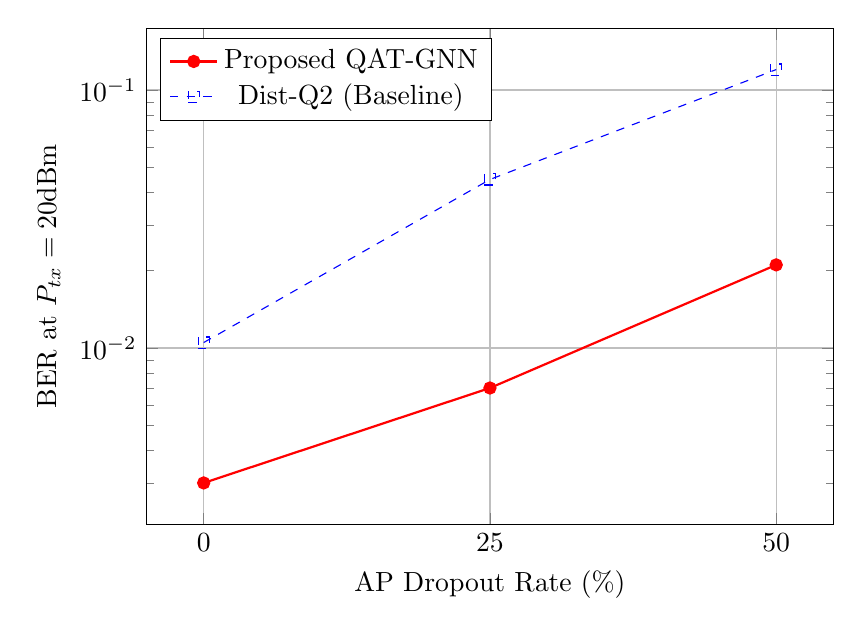
\begin{tikzpicture}
\begin{semilogyaxis}[
    xlabel={AP Dropout Rate (\%)},
    ylabel={BER at $P_{tx}=20$dBm},
    grid=major,
    xtick={0, 25, 50},
    width=0.85\linewidth,
    height=0.65\linewidth,
    legend style={at={(0.02,0.98)},anchor=north west}
]
\addplot[color=red, mark=*, thick] coordinates {(0, 0.0030) (25, 0.0070) (50, 0.0210)}; \addlegendentry{Proposed QAT-GNN}
\addplot[color=blue, mark=square, dashed] coordinates {(0, 0.0105) (25, 0.0450) (50, 0.1200)}; \addlegendentry{Dist-Q2 (Baseline)}
\end{semilogyaxis}
\end{tikzpicture}